\chapter{The COMET Experiment}\label{chapter2}

% \begin{markdown}
% ---

% - Description of the COMET experiment's goal, design with nice illustrations
%     + *Reference next chapter for geometry renderings*
%     + Signal and background:
%         + mu-e conv signal description
%         + **List of background sources**
% + CyDet:
%     + For simulation section, need to explain how CDC and CTH work, and how combined they enable mu--e conv measurement
%     - Detailed description of the CDC, which is crucial for the GAN section.
%      - Stereo angles
% + Phase alpha?

% - References: TDR, SINDRUM II, 

% ---

% + Requirements: high sensitivity to signal, efficient rejection of backgrounds
%  + -> Need intense muon beam, pulsed, and detector design must avoid backgrounds
% + TIMING of signal (muon lifetime)
% + Proton beam energy: why 8 Gev -> antiproton production
% + Intensity: beam current, beam power, POTs per second
% + Send backward-going secondaries to detector, discard the main part of secondaries (forward-going)
% + Curved solenoid + dipole field (by tilting coils, see Krikler)
% + Stopping target -> why Al
% + Bunch structure, extinction
% + Phase-I detectors: StrECAL and CyDet

% ---
% \end{markdown}

% Description and goals
COMET (COherent Muon-to-Electron Transition) is a future muon-beam experiment
designed to search for the muon-to-electron conversion
process~\cite{the_comet_collaboration_comet_2020}. It is currently under
construction at the Japan Proton Accelerator Research Complex (J-PARC) facility
in Tokai, Japan. The goal of COMET is to be \numprint{10000} times more
sensitive to $\mu$--$e$ conversion than the current world-leading limit set by
the SINDRUM II experiment~\cite{Bertl:2006up}. 

% Requirements
In order to reach these goals, the COMET experiment is designed with strict
requirements defined to make the conversion signal as clear as possible, while
efficiently rejecting background events. The most essential requirements are:
\begin{itemize}
    \item An intense muon source to probe the rare conversion process;
    \item A pulsed beam such that timing information can be used to reject backgrounds;
    \item Strict selection of charge and momentum of beam particles prior to
    reaching the detector.
\end{itemize}
These requirements and the design choices that were made to address them are
described in more detail in Section~\ref{Phase-I_requirements}.
% Later, go back to requirements and explain in more detail and then tell what
% the design choices were to address these requirements.

% Strategy
COMET is planned to run in a staged approach such that the properties of the
newly designed beam can be finely understood before making the measurement.
COMET Phase-I has a double purpose, each fulfilled by a distinct detector
systems. The StrECAL detector, composed of a straw-tube tracker and
electromagnetic calorimeter, will study the beam composition and timing
properties and increase our understanding of potential backgrounds. The
Cylindrical Detector, composed of a cylindrical drift chamber and a trigger
hodoscope, will perform a $\mu$--$e$ conversion search with a single-event
sensitivity (see Section~\ref{sec:SES}) of $3\times 10^{-15}$, a factor-100 improvement over SINDRUM II.
COMET Phase-II is a planned upgrade to Phase-I with higher beam intensity and
better background rejection via a longer momentum-selecting beamline. Phase-II
aims to improve on the single-event sensitivity of Phase-I by another factor of
$100$ to reach a single-event sensitivity of $2.6\times 10^{-17}$.

Figure~\ref{fig:comet_schematic} shows a top-down schematic view of the COMET
experiment, laying out the different sections that make up the beamline in
Phase-I and Phase-II. Note the addition of more momentum-selecting curved
solenoids in Phase-II for better rejection of high-momentum background-inducing
particles.

\begin{figure}
    \centering
    \begin{subfigure}[b]{0.46\textwidth}
    \centering
        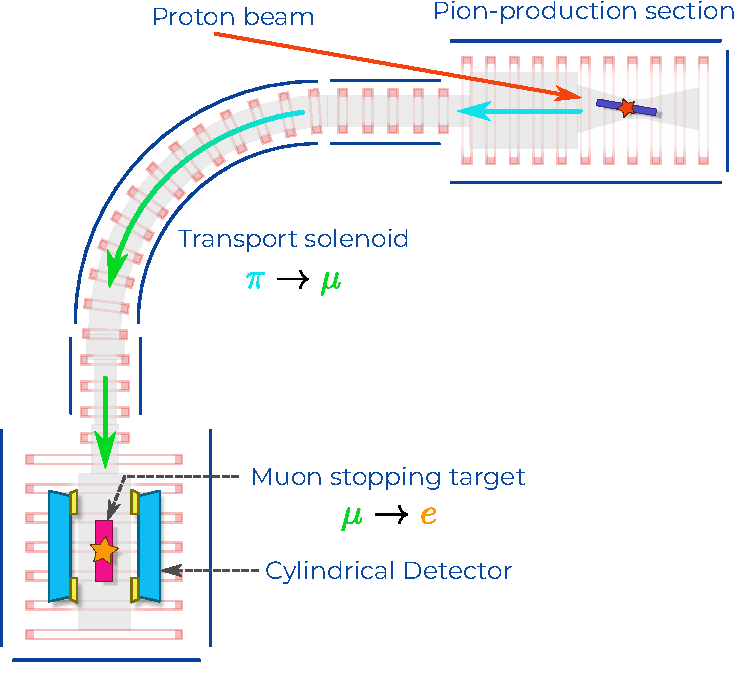
\includegraphics[width=\textwidth]{chapter2/comet_schematic_phase-I.pdf}
        \vspace{3cm}
        \caption{Phase-I with the Cylindrical Detector.}
    \end{subfigure}
    \hfill
    \begin{subfigure}[b]{0.49\textwidth}
        \centering
        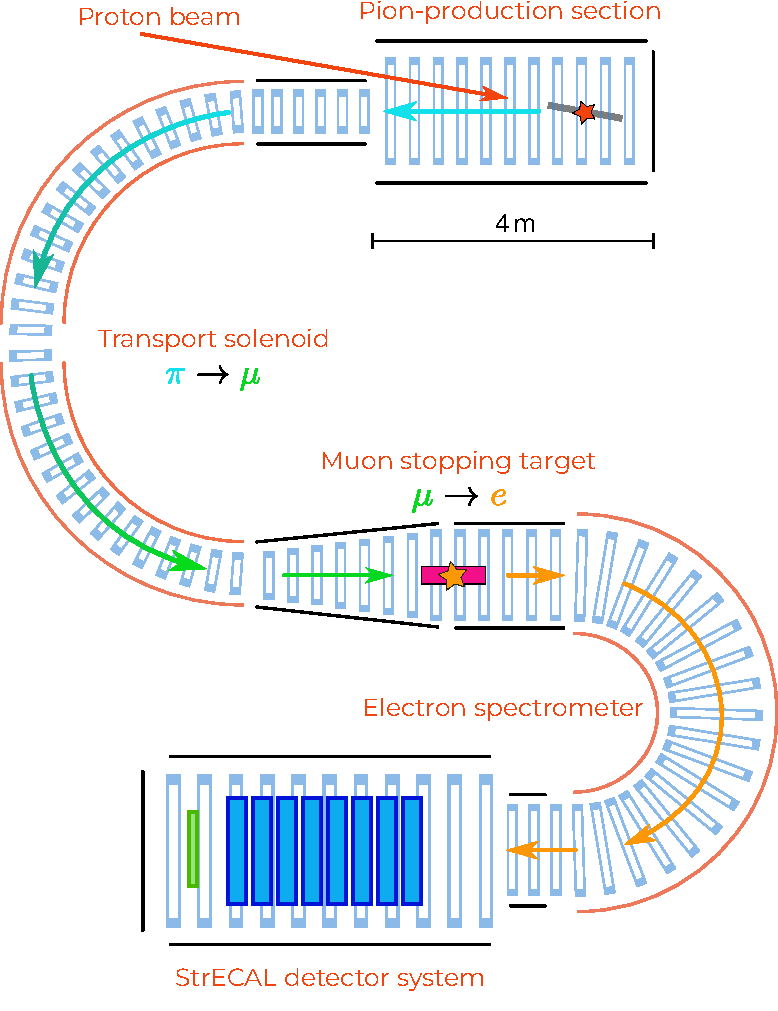
\includegraphics[width=\textwidth]{chapter2/comet_schematic.pdf}
        \caption{Phase-II.}
    \end{subfigure}
    \caption{ Schematic top-down view of the COMET experiment. The light blue
        rectangles along the whole beamline represent solenoids which guide the
        beam. Curved solenoids help to select momentum, as discussed in
        Section~\ref{sec:curved_solenoids}.}
    \label{fig:comet_schematic}
\end{figure}

% \footnote{For $\mu$--$e$ conversion searches, the single-event
% sensitivity (SES) is defined in terms of the fraction of muons captured by the
% target as $\mathrm{SES}(\mu^- N \rightarrow e^- N) = \frac{1}{N_\mu
% f_\mathrm{cap} f_\mathrm{gnd} A_{\mu\mathrm{--}e}}$}

\section{Proton beam}\label{sec:COMET_beam}
J-PARC provides a 8 \SI{8}{\GeV} proton beam 
The proton beam is provided by the J-PARC facility. It is a 

\section{Muon production}
% NOT REVIEWED:
Searching for $\mu$--$e$ conversion requires an intense source of muons. The
COMET experiment relies on the J-PARC accelerator facility to provide protons.
The proton beam hits a static graphite target to produce pions, which then decay
to muons. In order for the collision to produce a reasonable number of pions
while avoiding anti-proton production\footnote{
Anti-protons have the same charge as pions but travel more slowly for a given
momentum. Hence, they can produce delayed secondaries which hit the detector
system, which is a source of background as discussed in
Section~\ref{sec:delayed_backgrounds}. A beam energy of \SI{8}{\GeV} is the
lower limit above which anti-proton production becomes kinematically allowed.
}, the protons in the beam have a kinetic energy of \SI{8}{\GeV}. 


\section{Experimental backgrounds}\label{sec:backgrounds}
The COMET experiment is specifically designed to be sensitive to a $\mu$--$e$
conversion signal, i.e.\ to eliminate as many sources of background as possible
while making sure to notice the process if it does occur. 

Observing $\mu$--$e$ conversion requires the production of an intense source of
muons which must be bound to atomic nuclei. COMET uses a proton beam from the
J-PARC main ring.


The COMET experiment will produce a
muon beam and direct it toward a static aluminium target to slow down and stop
the muons. As discussed in Section~\ref{sec:sm_backgrounds}, a bound muon can
undergo decay in orbit (DIO) or nuclear capture. 

\section{Design requirements}

The design of the COMET experiment is heavily angled toward suppressing
backgrounds to the $\mu$--$e$ conversion signal. Understanding the background
sources and their properties is key in making sense of the experimental design.

\subsection{Curved solenoids}\label{sec:curved_solenoids}
Drift.

% The choice of target material directly influences how frequently high-energy
% electrons will be produced by these processes, and hence contributes in
% setting the maximum experimental sensitivity.

% This should go into the COMET section as these are specific to COMET and/or
% specifically addressed by the COMET design.
% Background events can be classified into three categories: intrinsic,
% beam-related, and cosmic ray-induced.

% Beam-related backgrounds come from impurities in the high-intensity muon beam.
% The specifics of the COMET beam and how these backgrounds are alleviated is
% discussed in Section~\ref{sec:COMET_beam}.

% Cosmic rays typically produce muons with a wide range of energies in the
% atmosphere which 